\section{Pandora/Larsoft Overview?}

\section{Motivation for improving the shower energy reconstruction}
Important for the selections. 
Need to correct for SCE.
\section{Overview/History of different methods used in SBND}
Linear Energy Tool. \newline
kGeVToElectrons:
\begin{itemize}
    \item Get hits associated with cluster.
    \item Loop over hits to get the charge whilst correcting or electron lifetime.
    \item Correct for recombination using a nominal fixed value of 0.64 (reference Ed's study showing it should be roughly this value) 
    \item Convert the collected charge to number of electrons using the calorimetry alg.
    \item Convert the number of electrons to Energy using the kGeVToElectrons scale factor. 
\end{itemize}
kGeVToElectrons correcting for SCE:
\begin{itemize}
    \item Use the modified box model.
    \item Not trivial to obtain a value for dE/dx.
    \item Assume dE/dx will be relatively constant. Calculate a nominal dE/dx by feeding in the nominal recombination value (0.64) and nominal E-Field (0.5) into the ModBox equation. 
    \item Attempt to correct for SCE, by finding the local E-field in the detector at the position of the hits/shower. Use this along with the nominal dE/dx and calculate a local value for the recombination. 
    \item Use the local recombination value when correcting the obtained charge. 
\end{itemize}

\section{Current method (ESTAR)}
The \textit{Shower ESTAR Energy tool} is the currently used method to reconstruct shower energy in SBND. It combines the ESTAR database along with the Modified Box recombination model. This approach was first used in the in ArgoNeuT experiment \cite{ArgoNeuT_ESTAR_paper}. The ESTAR database is provided by the National Institute of Standards and Technology (NIST) and gives the track length of electrons in liquid argon for energies ranging from 0.01 MeV to 1000 MeV \cite{ESTAR_Database}. The Modified Box recombination model is given by \begin{equation}\label{ModBox_eqn}
    \frac{dE}{dx} = \frac{\exp{(\frac{\beta}{\rho \mathcal{E}} W_{ion}.\frac{dQ}{dx}} - \alpha)}{\frac{\beta}{\rho \mathcal{E}}}
\end{equation}
where $\frac{dE}{dx}$ is the deposited energy per unit length, $\frac{dQ}{dx}$ is the deposited charge per unit length,  $\mathcal{E}$ is the electric field in the detector, $\rho$ is the density of liquid argon, $W_{ion} = 23.6$ eV which is the energy required to ionise an argon atom, $\alpha = 0.93 \pm 0.02$ and $\beta = 0.212 \pm 0.002$ (kV/cm)(g/cm$^2$)/MeV. The values for parameters $\alpha$ and $\beta$ are results from the ArgoNeuT experiment \cite{ArgoNeuT_recombination_paper}. 

The $\frac{dE}{dx}$ values are calculated by dividing the energy by the track length for each entry in the ESTAR database. The deposited charge, Q, is then found by using Equation (\ref{ModBox_eqn}) to find $\frac{dQ}{dx}$ and multiplying by the track length, dx. This now allows the deposited charge and energy to be related. If $\mathcal{E}$ in Equation \ref{ModBox_eqn} is taken to be a variable, the above process is repeated whilst iterating over a set values of $\mathcal{E}$. This results in a 3D curve relating both the deposited charge and electric field to energy as is shown in Figure (\ref{fig:ESTAR lookup curve}). The overall reconstruction chain is similar to that described in (???), but instead of directly converting the number of electrons using a scale factor, this lookup curve is used the interpolate the energy from the deposited charge and electric field. Electron lifetime correction are applied as before, however a direct recombination correction is not required as this has been accounted for in the lookup curve. 

\begin{figure}[hb]
    \centering
    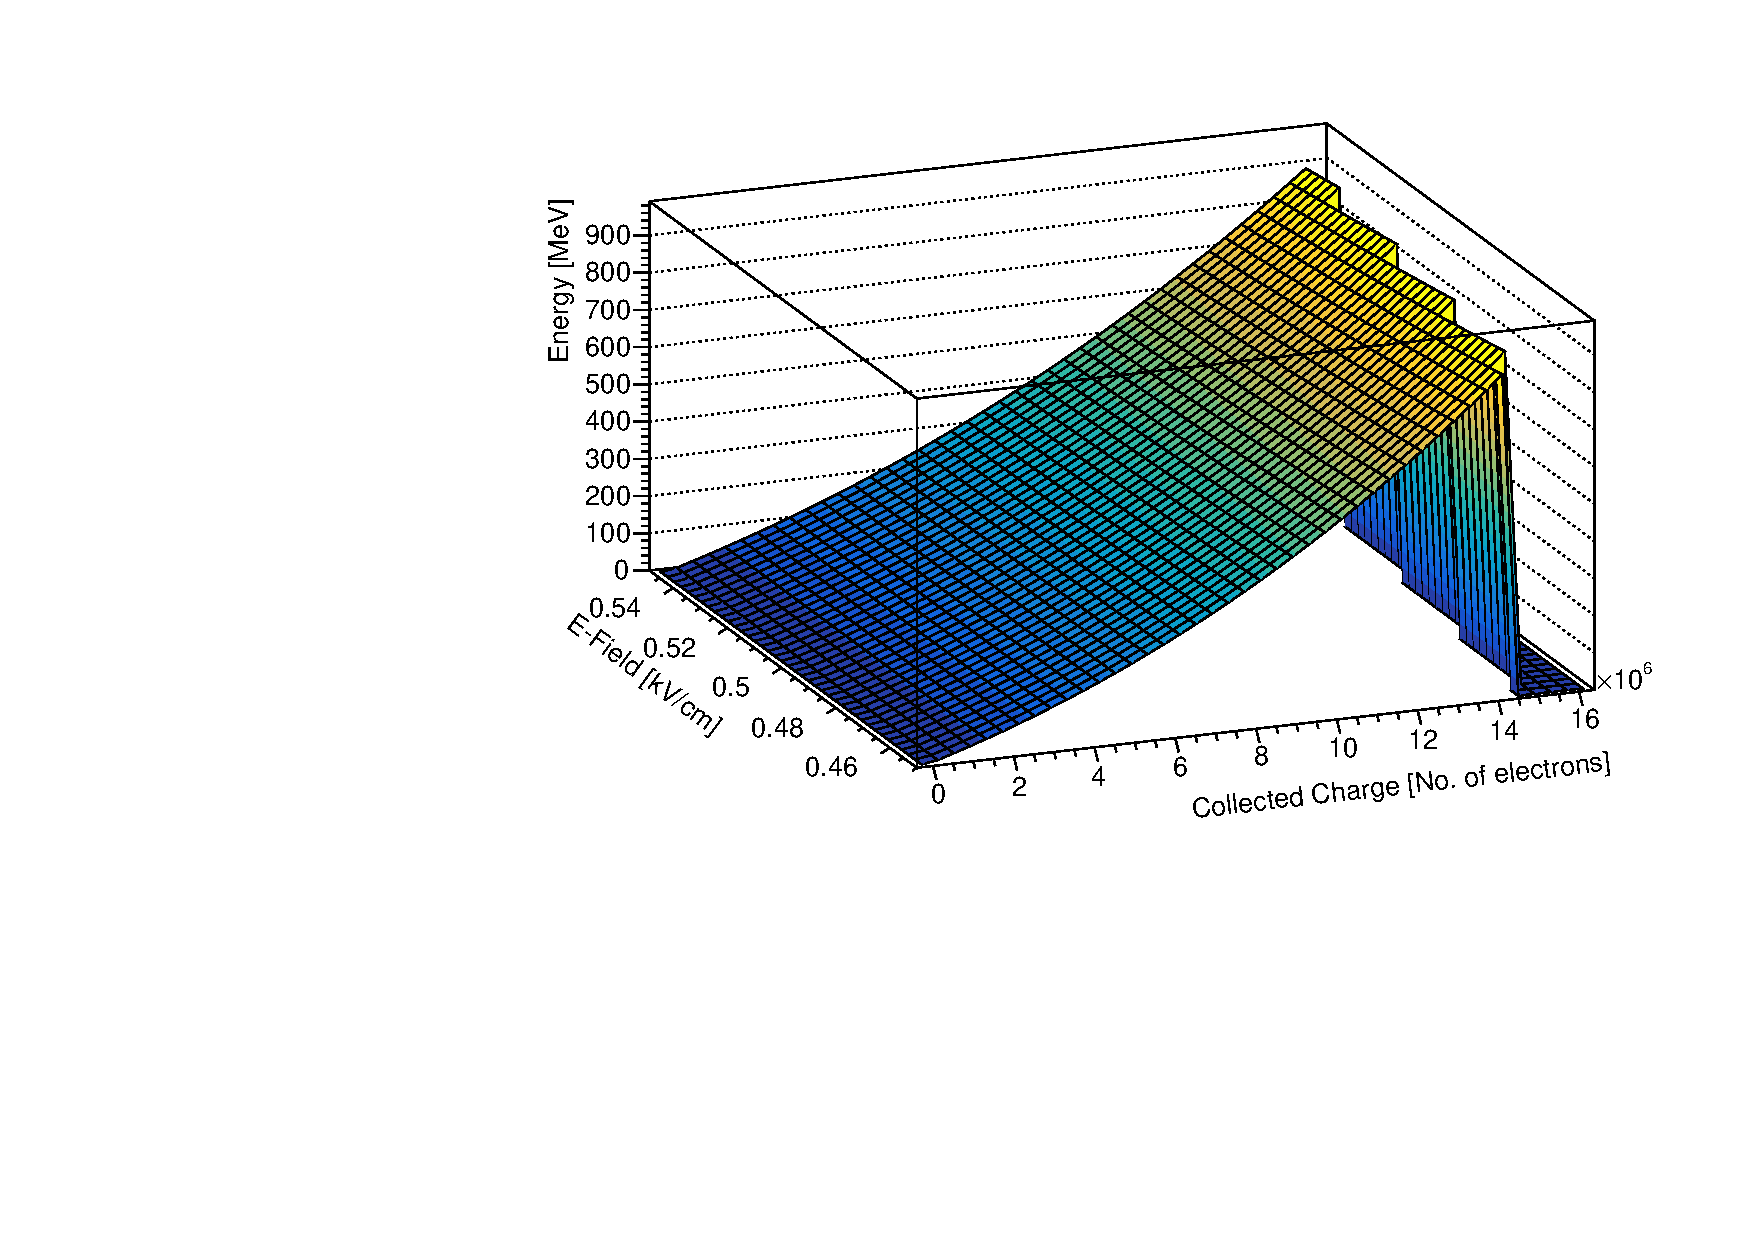
\includegraphics[width = 0.8\textwidth]{figures-chap4/ESTAR_lookup_curve.pdf}
    \caption{Caption}
    \label{fig:ESTAR lookup curve}
\end{figure}

To assess the performance of the \textit{Shower ESTAR Energy tool}, the the reconstructed energy of each hit was summed up for all the hits in a shower. This was compared the sum of the true energy of all the hits.

ESTAR: 
\begin{itemize}
    \item Use ESTAR database in conjunction with ModBox equation to create lookup curve of collected charge vs energy. Inspired by method used in ArgoNeuT 
    \item This lookup curve has recombination correction 'baked-in'. Same method as kGeVToElectrons (obviously not double correcting for recombination), but instead of using scale factor to convert to energy, we use the lookup curve.
    \item To correct for the SCE, treat the E-Field in the ModBox model as a variable instead of a constant. Now produce a 3D lookup curve of collected charge vs E-Field vs energy. When converting the hits to energy, we use the lookup curve to interpolate the energy from from the collected charge and the local E-Field of the hit.  
\end{itemize}

\section{Summary + outstanding issues etc}

Energy Reco - Things to include.

\begin{itemize}
	\item Motivation (why do we care?)
	\item Explain choices - use vertex sample because it helps pandora. Only considering largest shower (most hits) from each event. 
	\item Overview of the very first method that was being used. Use muons to generate lookup curve. Get linear relationship between deposited charge and energy. Plagiarise Dom's thesis on this..  
	\item Change method so we convert the deposited charge to number of electrons and then convert the number of electrons to energy using the appropriate calibration/scale factors. Apply correction for electron lifetime as before and also correct for recombination. Previously recombination correction was 'baked' into the look-up curve. No way to correct for it directly - whenever we would change the \textit{physics} we would need to regenerate the look-up curve. With this method it's possible to tweak the recombination correction directly. 
	\item Not straight forward to calculate the recombination directly - let's use and average value for all showers - explain recombination study. 
	\item Consider SCE - explain what SC is.
	\item How do we account for SCE? Get map of the E-field in the detector (not uniform because of SC). Using the nominal value of the recombination and E-field, calculate a nominal dE/dx (not straightforward to calculate directly) which we assume remains constant. Can now use the Modified Box model to weak the recombination correction by feeding the local E-field (which depends on the location in the detector) back into the modified box model. Finally, find the (charge weighted) centre of the shower using the space points and use the local E-field at this point to calculate the recombination factor at this location. 
	\item No reason we can't do a per-hit analysis. Redo everything as before for each individual hit and then sum to get the energy of the shower. Should give better results since the recombination correction is more accurate now. 
	\item We have the ability to attempt to correct for the SCE as mentioned, but are limited by not knowing the dE/dx. So correcting the SCE without this caveat becomes tricky.. Try a new approach developed by ArgoNeuT - use the ESTAR database. The ESTAR database gives us the stopping power of (dE/dx) of electrons in various materials (including lAr) in a range of energies and is based partly from data. Combining this with the modified box recombination model, we can again create a lookup curve of energy vs deposited charge with the recombination correction baked in. Since the modified box model depends on the E-Field, we can treat this as a variable and create a 3D lookup curve of energy vs E-Field vs deposited charge which will allow us to correct for SC. 
	\item \textit{True} energy debacle.. We have the true energy of the showering particle and the true energy of all the hits in a given shower. Originally we used the true energy of the showering particle for comparison (in hindsight this seems like a stupid idea..) and the kGeVtoElectrons method clearly outperformed ESTAR. Swapping to the true hit energies, ESTAR does better. What was happening (i think) is that kGeVToElectrons over estimates the hit energies, so when comparing with the true showering particle this method give a better result because we're papering over the cracks due to the pattern recognition and hit inefficiencies. ESATR method gives a better result for individual hit energies so highlights the failing of the patter rec and hit inefficiencies when comparing with the showering particle. 
	\item Why some results are shit.. Pandora pattern recognition (clustering) is far from perfect - can use Pandora in cheating mode to overcome this. There are hit inefficiencies i.e. hit reconstruction isn't perfect - haven't ever \textit{cheated} this, dunno if it's an option. The actual impact from SC is pretty minimal but it also impacts Pandora's pattern recognition. This can a have a big impact - what Pandora initially recognised as one big shower may be interpreted as 2+ smaller showers after applying SC (and vice-versa). Also, an object classified as a shower may instead be classified as a track after applying SC. Since we're only considering the largest shower for each event, this effects mean SC can appear to have a impact. 
\end{itemize}
